\documentclass[12pt,letterpaper]{article}

\usepackage[utf8]{inputenc}
\usepackage[spanish]{babel}
\usepackage{times}
\usepackage[left=3cm,top=2.5cm,bottom=2.5cm,right=2.5cm]{geometry}
\usepackage{graphicx}
\title{EV\_ 2\_ 2\_ Explicar\_ los\_ arreglos\_ y\_ parámetros\_ de\_ los\_ Amplificadores\_ Clase\_ A.}


\begin{document}
\maketitle




\paragraph{ UNIVERSIDAD POLITÉCNICA DE LA ZONA METROPOLITANA DE GUADALAJARA}

\
\begin{figure}[h!]
\begin{center}


\includegraphics[scale=0.8]{Upzmg.png} 
\label{Upzmg}


\end{center}
\end{figure}


\

\large{Perez de Alba Santiago Eduardo.\\
Fecha: 24 de septiembre del 2019.
\

Curso: Sep-Nov 2019.

\
Carrera: Ingeniería en Mecatronica.\

Docente: Moran Garabito Carlos Enrique}

\newpage

\section{Marco teórico:}
\

¿Qué es un Amplificador?
\

Son aquellos cuyas etapas de potencia consumen corrientes altas y continuas de su fuente de alimentación, independiente de si existe señal o no.
\

\

Estos proporcionan la máxima potencia de salida para una selección dada de dispositivo activo, realmente se habla de transistores con salidas RF de mas de 1W. Los Amplificadores tienen limites físicos de corriente que puede proporcionar y de tension que puede mantener

\

\

Los amplificadores operacionales de clase A poseen baja distorsión de amplitud y una excelente linealidad. Esté esta polarizado de tal forma que la corriente por el colector fluye durante el ciclo completo de la señal de entrada. El amplificador reproduce toda la señal de entrada, la corriente de colector es distinta de cero todo el tiempo, lo cual se considera muy ineficiente, ya que para señal cero en la entrada, se tiene un \textit{$I_{CQ}$}$>$0, luego el transistor disipa la potencia.

\

El amplificador clase A tiene distintas configuraciones, una de ella es el Amplificador de emisor común.

\

\begin{figure}[h!]
\begin{center}

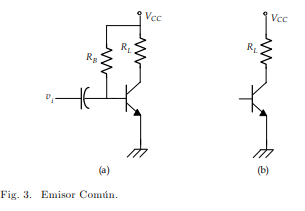
\includegraphics[scale=0.8]{Emisor comun.png}
\caption{Amplificador-Emisor común}
\end{center}

\end{figure}
 
\
Esta puede ser muy simple, ya que se hace la resistencia del emisor $R_E$=0. Se selecciona $R_L$ para máxima potencia potencia de salida, lo que implica que la recta de carga de CA debe pasar por la curva $P_{CEMAX}$

La eficiencia de los Clase A puede ser mas grande que el 50\%; por ejemplo, para una onda cuadrada puede llegar al 100\%
\

\subparagraph{Caracteristicas:}

\

Estos tienen un inconveniente ya que generan una fuerte y constante emisión de calor. Sin embargo, los transistores de salida están siempre a una temperatura fija y sin alteraciones.




\





\end{document}